%%% Содержимое слайдов

\frame[plain]{\titlepage} % Титульный слайд

%-------------------------------------------------------------------------------

\section{Разработка виртуальной инфраструктуры для реализации облачных услуг}

\begin{frame}
\frametitle{\insertsection}
%\framesubtitle{Требования}
Требования:
\begin{itemize}
	\item устранение единых точек отказа (резервные линки, RAID)
	\item защита от недоброжелателей (DDoS, флуд)
	\item \textbf{использование свободного ПО по возможности}
	\item документирование
	\item автоматизация
	\item разработка эффективных тарифных планов хостинга и VPS
	\item использование в бизнесе
\end{itemize}
\end{frame}

\begin{frame}
\frametitle{\insertsection}
%\framesubtitle{Подпункт 2}
Возможности:
\begin{itemize}
	\item весьма ограниченный бюджет
	\item всего один админ, он же архитектор (некрасиво звучит этот пункт)
	\item отсутствие опыта работы с виртуализацией
	\item желание что-то построить
\end{itemize}
\end{frame}

%-------------------------------------------------------------------------------

\section{Общая схема инфраструктуры}

\begin{frame}
\frametitle{\insertsection}
%\framesubtitle{Подпункт 1}
\begin{figure}[h]
	\begin{center}
		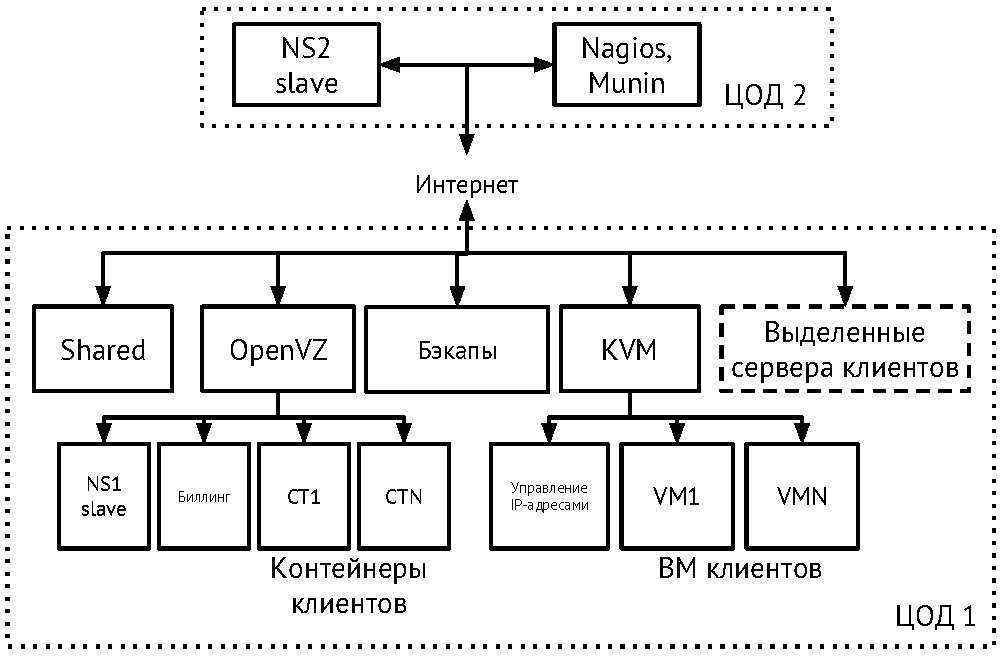
\includegraphics[width=\linewidth]{infrast-scheme}
	 \end{center}
\end{figure}
\end{frame}

%-------------------------------------------------------------------------------

\section{Используемое свободное ПО}

\begin{frame}
\frametitle{\insertsection}
%\framesubtitle{Подпункт 2}
\begin{itemize}
	\item Linux
	\item мониторинг
	\item виртуализация
	\item автоматизированное управление конфигурациями
	\item скрипты, много скриптов
	\item стандартный стек хостинга
	\item вирусы и malware на хостинге
	\item панели для пользователей виртуальных серверов
\end{itemize}
\end{frame}

%-------------------------------------------------------------------------------

\section{ОС}

\begin{frame}
\frametitle{\insertsection}
\framesubtitle{CentOS 7 (GPL)}
\begin{itemize}
	\item гораздо популярнее на серверах чем Windows/FreeBSD
	\item изобилие серверного ПО
	\item поддержка 6-10 лет (обновление пакетов, исправление уязвимостей и багов)
	\item бесплатно
	\item простая сборка пакетов
	\item драйвера
	\item много документации
\end{itemize}
\end{frame}

%-------------------------------------------------------------------------------

\section{Мониторинг}

\begin{frame}
\frametitle{\insertsection}
\framesubtitle{Nagios → Icinga2 (GPLv2)}
\begin{figure}[h]
	\begin{center}
		\begin{multicols}{2}
		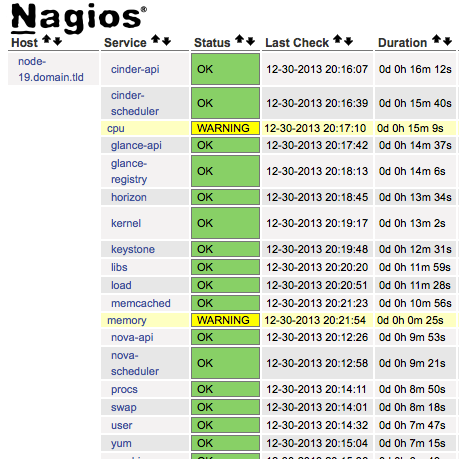
\includegraphics[width=\linewidth]{nagios} \pause \\
		\uncover<2->{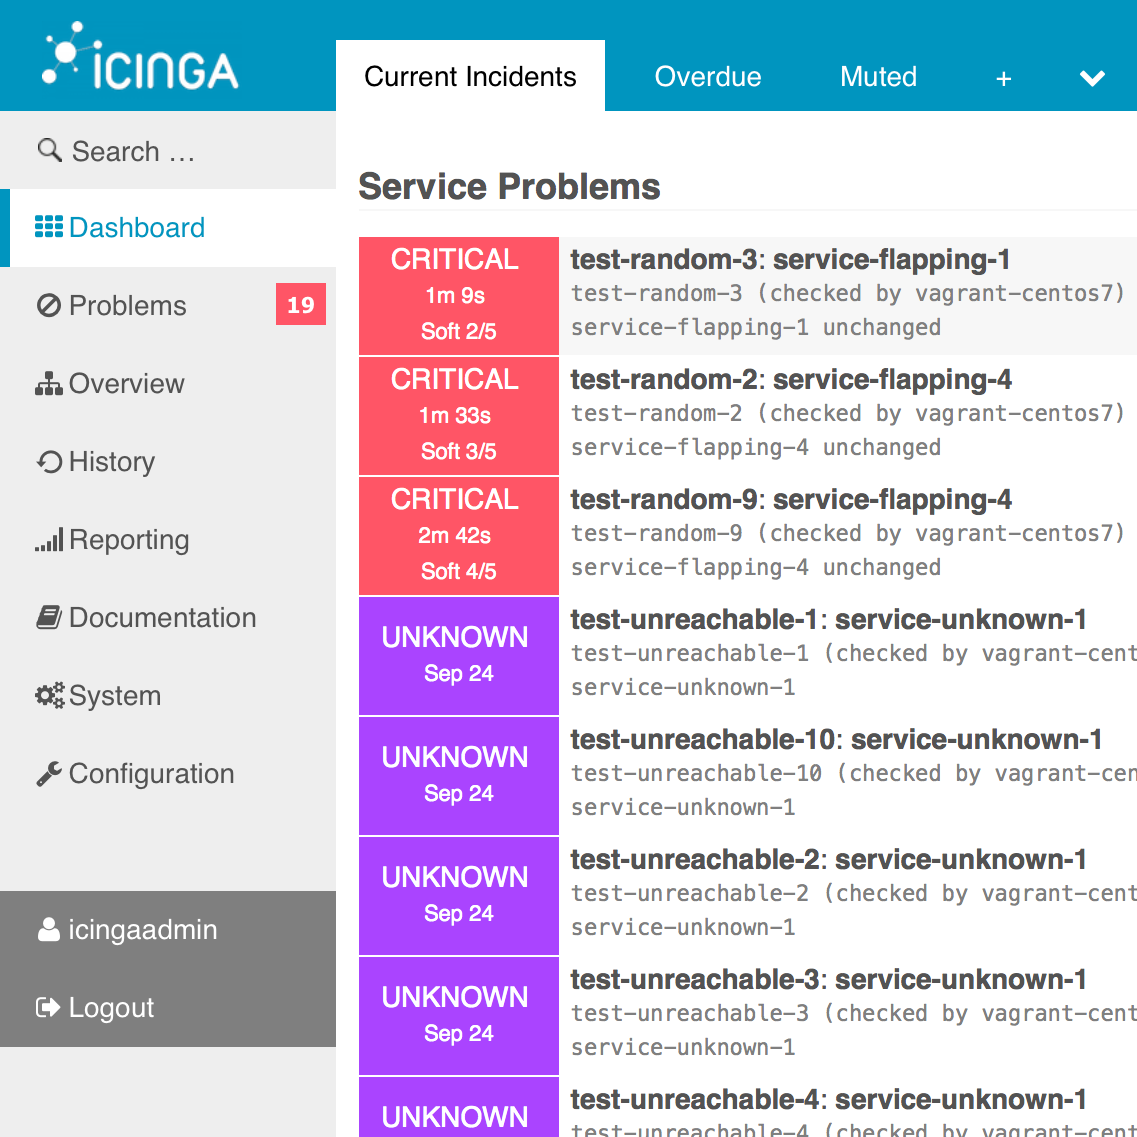
\includegraphics[width=\linewidth]{icinga2}}
		\end{multicols}
	 \end{center}
\end{figure}
\end{frame}

\begin{frame}
\frametitle{\insertsection}
\framesubtitle{Munin (GPL)}
\begin{figure}[h]
	\begin{center}
		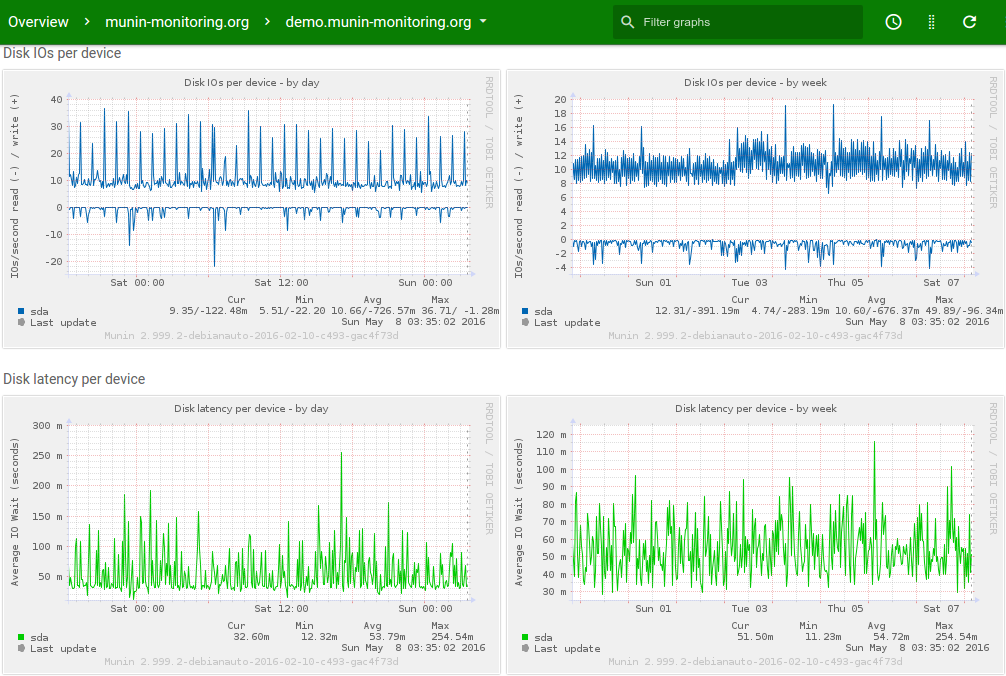
\includegraphics[width=\linewidth]{munin}
	 \end{center}
\end{figure}
\end{frame}

%-------------------------------------------------------------------------------

\section{Управление конфигурациями}

\begin{frame}
\frametitle{\insertsection}
\framesubtitle{Ansible (GPL)}
\begin{figure}[h]
	\begin{center}
		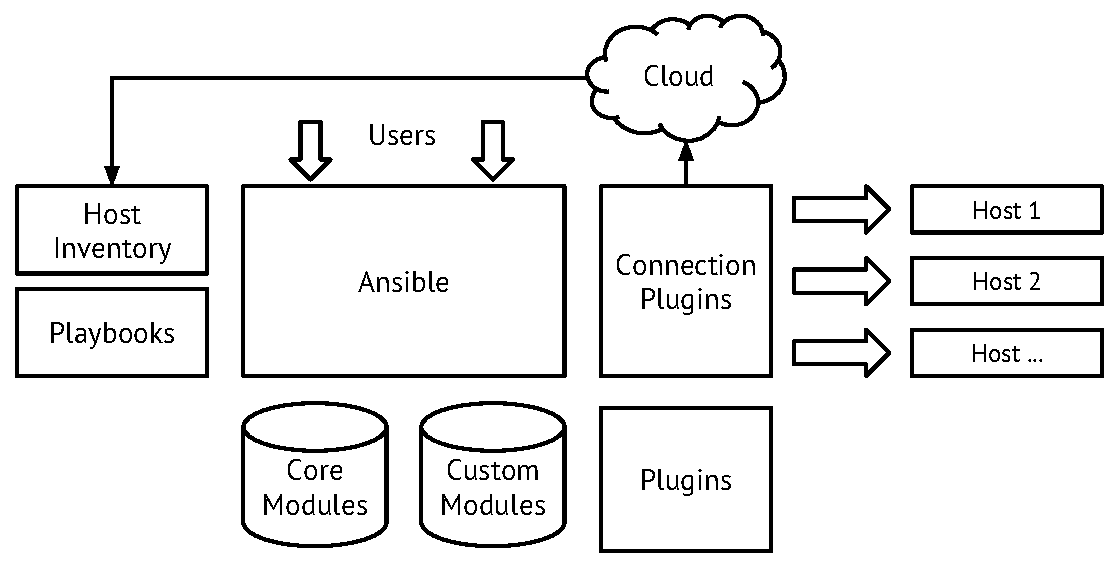
\includegraphics[width=\linewidth]{ansible}
	 \end{center}
\end{figure}
\end{frame}

%-------------------------------------------------------------------------------

\section{Свободное ПО}

\begin{frame}
\frametitle{\insertsection}
%\framesubtitle{Подпункт 2}
\begin{enumerate}
	\item Элемент 1
	\uncover<2->{\item Элемент 2}
	\uncover<3->{\item Элемент 3*}
\end{enumerate}
\begin{figure}[h]
	\begin{center}
		\begin{multicols}{2}
		
\includegraphics[width=0.3\linewidth]{one} \pause \\
		\uncover<2->{
\includegraphics[width=0.3\linewidth]{two}} \pause \\
		\end{multicols}
		\uncover<3->{
\includegraphics[width=0.15\linewidth]{three}}
	 \end{center}
\end{figure}
\vfill
\footnotesize{* Какая-то сноска}
\end{frame}

%-------------------------------------------------------------------------------

\section{Пункт 3}

\begin{frame}
\frametitle{\insertsection}
\framesubtitle{Подпункт 1}
\begin{itemize}
	\begin{multicols}{2}
	\item Элемент 1
	\item Элемент 1
	\item Элемент 1
	\item Элемент 1
	\item Элемент 1
	\item Элемент 1 \pause \columnbreak
	\item Элемент 2
	\item Элемент 2
	\item Элемент 2
	\end{multicols}
\end{itemize}
\end{frame}

\begin{frame}
\frametitle{\insertsection}
\framesubtitle{Подпункт 2}
\begin{itemize}
	\item Элемент 1
	\begin{itemize}
		\item Подэлемент 1
		\item Подэлемент 2
		\item Подэлемент 3
	\end{itemize}
	\item Элемент 2
	\item Элемент 3
\end{itemize}
\end{frame}

%-------------------------------------------------------------------------------

\section{Выводы}

\begin{frame}
\frametitle{\insertsection}
\begin{itemize}
	\item Элемент 1
	\item Элемент 2
	\item Элемент 3
	\item Элемент 4
\end{itemize}
\end{frame}

%-------------------------------------------------------------------------------

\section{Информационные источники}

\begin{frame}
\frametitle{\insertsection}
\begin{itemize}
	\item Источник 1: \url{http://1.example.com}
	\item Источник 2: \url{http://2.example.com}
	\item Источник 3: \url{http://3.example.com}
	\item Источник 4: \url{http://4.example.com}
\end{itemize}
\end{frame}

%-------------------------------------------------------------------------------

\frame[plain]{\titlepage} % Титульный слайд
